\subsubsection{Suite de Fibonacci}



La \textbf{suite de Fibonacci} permet de décrire par exemple l'évolution d'une population de lapins par exemple.

\begin{center}
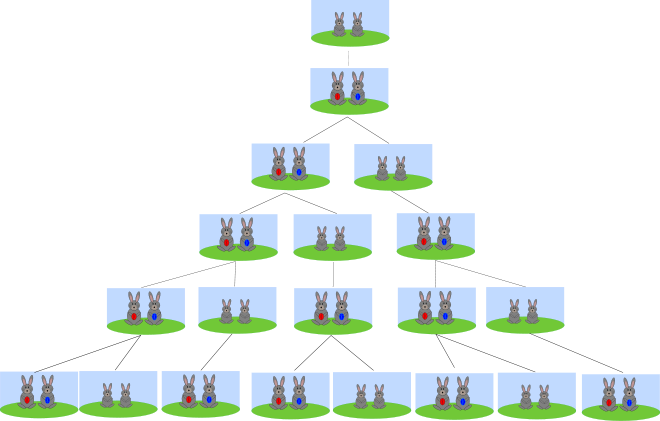
\includegraphics[width=0.6\textwidth]{fibonacci.png}
\end{center}

Cette suite est définie de la façon suivante : 

\begin{align*}
\left\{
\begin{array}{c}
F_0=0\\
\\
F_1=1\\
\\
F_{n+2}=F_{n+1}+F{n}\\
\end{array}
\right.
\end{align*}





\question{Écriture sous Python \texttt{fib_it(n:int)->F(n)} calculant le terme de rang $n$ ($F_n$) de la suite de Fibonacci par une méthode itérative.}



\begin{lstlisting}
def fib_it(n):
    u=0
    v=1
    if n<=1:
        v=n
    for k in range(2,n+1):
        u,v=v,u+v
    return v
\end{lstlisting}

\question{Écriture sous Python \texttt{fib_rec(n:int)->F(n)} calculant le terme de rang $n$ ($F_n$) de la suite de Fibonacci par une méthode recursive.}

\begin{lstlisting}
def fib_rec(n):
    u=0
    v=1
    if n<=1:
        v=n
    for k in range(2,n+1):
        u,v=v,u+v
    return v
\end{lstlisting}